\documentclass[tikz,border=5pt]{standalone}
\usepackage{tikz}
\usetikzlibrary{calc}

\begin{document}

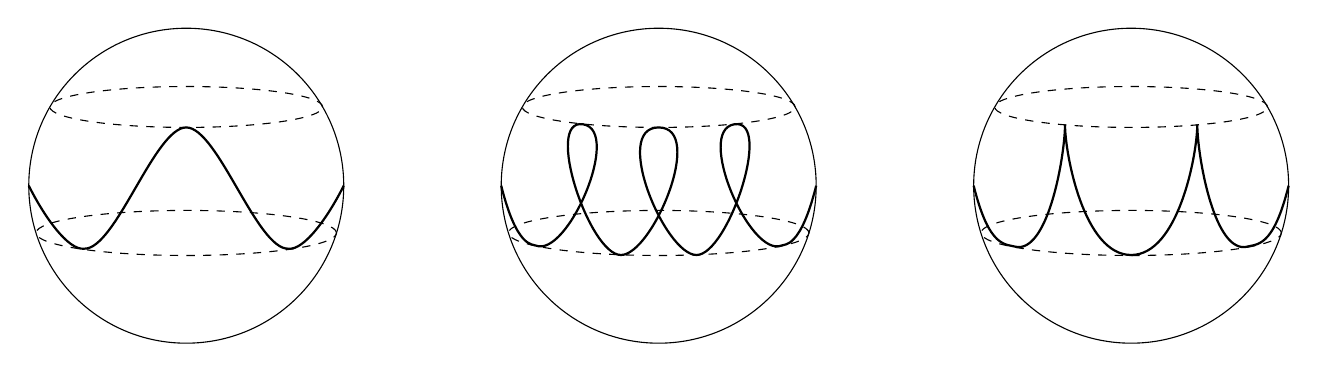
\begin{tikzpicture}[scale=2]

% parameters
\def\R{1}
\def\thetaone{-17.457}
\def\thetatwo{30}


% nutation curve (a)
\begin{scope}[xshift=-3cm]
\draw (0,0) circle (\R);
\draw[dashed] (0,-0.3) ellipse ({\R*cos(\thetaone)} and {0.15*\R*cos(\thetaone)});
\draw[dashed] (0,0.5) ellipse ({\R*cos(\thetatwo)} and {0.15*\R*cos(\thetatwo)});
\draw[thick,-] (-1,0)
.. controls (-0.9,-0.2) and (-0.75,-0.41) .. (-0.65,-0.4)
.. controls (-0.45,-0.41) and (-0.2,0.37) .. (0,0.37)
.. controls (0.2,0.37) and (0.45,-0.41) .. (0.65,-0.4)
.. controls (0.75,-0.41) and (0.9,-0.2) .. (1,0);
\end{scope}

% nutation curve (b)
\begin{scope}[xshift=0cm]
\draw (0,0) circle (\R);
\draw[dashed] (0,-0.3) ellipse ({\R*cos(\thetaone)} and {0.15*\R*cos(\thetaone)});
\draw[dashed] (0,0.5) ellipse ({\R*cos(\thetatwo)} and {0.15*\R*cos(\thetatwo)});
\draw[thick,-] (-1,0)
.. controls (-0.9,-0.4) and (-0.8,-0.37) .. (-0.78,-0.38)
.. controls (-0.58,-0.46) and (-0.23,0.35) .. (-0.48,0.39)
.. controls (-0.73,0.43) and (-0.44,-0.44) .. (-0.24,-0.44)
.. controls (-0.04,-0.44) and (0.3,0.37) .. (0,0.37)
.. controls (-0.3,0.37) and (0.04,-0.44) .. (0.24,-0.44)
.. controls (0.44,-0.44) and (0.73,0.43) .. (0.48,0.39)
.. controls (0.23,0.35) and (0.58,-0.46) .. (0.78,-0.38)
.. controls (0.8,-0.37) and (0.9,-0.4) .. (1,0);
\end{scope}

% nutation curve (c)
\begin{scope}[xshift=3cm]
\draw (0,0) circle (\R);
\draw[dashed] (0,-0.3) ellipse ({\R*cos(\thetaone)} and {0.15*\R*cos(\thetaone)});
\draw[dashed] (0,0.5) ellipse ({\R*cos(\thetatwo)} and {0.15*\R*cos(\thetatwo)});
\draw[thick,-] (-1,0)
.. controls (-0.9,-0.4) and (-0.8,-0.37) .. (-0.72,-0.39)
.. controls (-0.52,-0.4) and (-0.42,0.2) .. (-0.42,0.39)
.. controls (-0.42,0.2) and (-0.3,-0.44) .. (0,-0.44)
.. controls (0.3,-0.44) and (0.42,0.2) .. (0.42,0.39)
.. controls (0.42,0.2) and (0.52,-0.4) .. (0.72,-0.39)
.. controls (0.8,-0.37) and (0.9,-0.4) .. (1,0);
\end{scope}

\end{tikzpicture}

\end{document}